\documentclass[a4paper,10pt]{article}

\usepackage[T1]{fontenc}
\usepackage[utf8]{inputenc}
\usepackage{graphicx}
\usepackage{xcolor}
\usepackage{fourier}
\usepackage{caption}
\usepackage{subcaption}

\usepackage{tgtermes}

\usepackage[
pdftitle={Statistical Machine Learning}, 
pdfauthor={Inez Wijnands \& Guido Zuidhof, Radboud University Nijmegen},
colorlinks=true,linkcolor=blue,urlcolor=blue,citecolor=blue,bookmarks=true,
bookmarksopenlevel=2]{hyperref}
\usepackage{amsmath,amssymb,amsthm,textcomp}
\usepackage{enumerate}
\usepackage{multicol}
\usepackage{tikz}

\usepackage{geometry}
\geometry{total={210mm,297mm},
left=25mm,right=25mm,%
bindingoffset=0mm, top=20mm,bottom=20mm}

\numberwithin{equation}{section} % Number equations within sections (i.e. 1.1 instead of 1)
\numberwithin{figure}{section} % Number figures within sections (i.e. 1.1 i/o 1)
\numberwithin{table}{section} % Number tables within sections (i.e. 1.1 i/of 1)

\linespread{1.35}

\newcommand{\linia}{\rule{\linewidth}{0.5pt}}

% custom theorems if needed
\newtheoremstyle{mytheor}
    {1ex}{1ex}{\normalfont}{0pt}{\scshape}{.}{1ex}
    {{\thmname{#1 }}{\thmnumber{#2}}{\thmnote{ (#3)}}}

\theoremstyle{mytheor}
\newtheorem{defi}{Definition}

% my own titles
\makeatletter
\renewcommand{\maketitle}{
\begin{center}
\vspace{2ex}
{\huge \textsc{\@title}}
\vspace{1ex}
\\
\linia\\
\@author  \@date
\vspace{4ex}
\end{center}
}
\makeatother
%%%

% custom footers and headers
\usepackage{fancyhdr,lastpage}
\pagestyle{fancy}
\lhead{}
\chead{}
\rhead{}
\lfoot{Assignment \textnumero{} 2}
\cfoot{}
\rfoot{Page \thepage\ /\ \pageref*{LastPage}}
\renewcommand{\headrulewidth}{0pt}
\renewcommand{\footrulewidth}{0pt}
%

% code listing settings
\usepackage{listings}
\lstset{
    language=Python,
    basicstyle=\ttfamily\small,
    aboveskip={1.0\baselineskip},
    belowskip={1.0\baselineskip},
    columns=fixed,
    extendedchars=true,
    breaklines=true,
    tabsize=4,
    prebreak=\raisebox{0ex}[0ex][0ex]{\ensuremath{\hookleftarrow}},
    frame=lines,
    showtabs=false,
    showspaces=false,
    showstringspaces=false,
    keywordstyle=\color[rgb]{0.627,0.126,0.941},
    commentstyle=\color[rgb]{0.133,0.545,0.133},
    stringstyle=\color[rgb]{01,0,0},
    numbers=left,
    numberstyle=\scriptsize\ttfamily,
    stepnumber=1,
    numbersep=10pt,
    captionpos=t,
    escapeinside={\%*}{*)}
}

%%%----------%%%----------%%%----------%%%----------%%%

\begin{document}

\title{Statistical Machine Learning \\ Assignment 2}

\author{Inez Wijnands (s4149696) \& Guido Zuidhof (s4160703)\\ Radboud University Nijmegen\\}

\date{04/11/2015}

\maketitle

\noindent \textit{The entire code listing is in a separate file. The listings shown here are merely code snippets}.\vspace{-0.5cm}
\section{Sequential learning}
\subsection{Obtaining the prior}
\begin{enumerate}
	\item \begin{align}
			\boldsymbol{\tilde \Lambda}_{a,b} &= \boldsymbol{\tilde \Sigma}_{a,b}^{-1} \\
			&= \newcommand*{\temp}{\multicolumn{1}{c|}{}} 
				 \begin{pmatrix}
					60&50&\temp&-48&38\\ 
					50&50&\temp&-50&40\\ \cline{1-5} 
					-48&-50&\temp&52.4&-41.4 \\
					38&40&\temp&-41.4&33.4
				\end{pmatrix}
		\end{align}\\\\
		Using the precision matrix $\boldsymbol{\tilde \Lambda}$ we can use equations 2.69, 2.73 and 2.75 from Bishop to obtain the mean and covariance of the conditional distribution $p([x_1,x_2]^T|x_3 = x_4 = 0)$.\\
		\begin{align}
			\boldsymbol{\Sigma}_p &= \boldsymbol \Lambda_{aa}^{-1} \tag{2.73 from Bishop}\\
			\boldsymbol \Lambda_{aa} &= \begin{pmatrix} 60 & 50 \\ 50 & 50 \end{pmatrix}\\
			\boldsymbol{\Sigma}_p &= \begin{pmatrix} 0.1 & -0.1 \\ -0.1 & 0.12 \end{pmatrix}
		\end{align}
		\begin{align}
			\boldsymbol{\mu}_p = \boldsymbol{\mu}_{a | b} = \boldsymbol{\mu}_a - \boldsymbol{\Lambda}_{aa}^{-1}\boldsymbol{\Lambda}_{ab}(\boldsymbol{x}_b - \boldsymbol{\mu}_b) \tag{2.75 from Bishop}
		\end{align}
		We can fill in this equation, since $\boldsymbol {\tilde \mu}$ and $\boldsymbol x_b$ (the second partition of $\boldsymbol x$) are known.
		\begin{align}
			\boldsymbol{\mu}_p &=
			\begin{pmatrix} 1\\ 0 \end{pmatrix}-
			\begin{pmatrix} 60 & 50 \\ 50 & 50 \end{pmatrix}^{-1}
			\begin{pmatrix} -48 & 38\\ -50 & 40 \end{pmatrix}
			(\begin{pmatrix} 0\\ 0 \end{pmatrix}-
			\begin{pmatrix} 1\\ 2 \end{pmatrix}) \\
			&= \begin{pmatrix} 1\\ 0 \end{pmatrix}-
			\begin{pmatrix} 0.1 & -0.1 \\ -0.1 & 0.12 \end{pmatrix}
			\begin{pmatrix} -48 & 38\\ -50 & 40 \end{pmatrix}
			(\begin{pmatrix} 0\\ 0 \end{pmatrix}-
			\begin{pmatrix} 1\\ 2 \end{pmatrix}) \\
			&= \begin{pmatrix} 0.8\\ 0.8 \end{pmatrix}
		\end{align}
	\item Using the prior $\boldsymbol \mu_p$ and $\boldsymbol \Sigma_p$, we used the numpy-equivalent in Python for the MATLAB-function \verb|mvnrnd| to obtain the $\boldsymbol \mu_t$ we used for the remainder of this assignment:
		\begin{verbatim}
			np.random.multivariate_normal(mu_p, sigma_p, 1)
		\end{verbatim}
		This resulted in:
		\begin{equation}
			\boldsymbol\mu_t = \begin{pmatrix} 0.28584241 \\ 1.42626702\end{pmatrix}
		\end{equation}
	\item The probability density is highest at the mean (as illustrated in Figure 1.1). The density decreases quickly as both x and y change, but less so when $x$ XOR $y$ change. In $\boldsymbol \Sigma_p$, the values for the $x$ XOR $y$ are lower, so this is consistent with our density plot.
		\begin{figure}[h!]
   			\centering
   			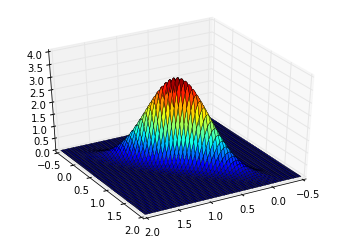
\includegraphics{probdens.png}\vspace{-0.2cm}
   			\caption{\vspace{-0.2cm} The probability density of the distribution.}
  		\end{figure}
\end{enumerate}
\subsection{Generating the data}
\begin{enumerate}
	\item
\end{enumerate}
\subsection{Sequential learning algorithms}
\begin{enumerate}
	\item
	\item
\end{enumerate}

\section{The faulty lighthouse}
\subsection{Constructing the model}
\begin{enumerate}
	\item 
	\item 
	\item
	\item
\end{enumerate}
\subsection{Generate the lighthouse data}
\begin{enumerate}
	\item
	\item 
\end{enumerate}
\subsection{Find the lighthouse}
\begin{enumerate}
	\item
	\item 
	\item 
\end{enumerate}
\end{document}
